\begin{answer}
Unregularized loss curves

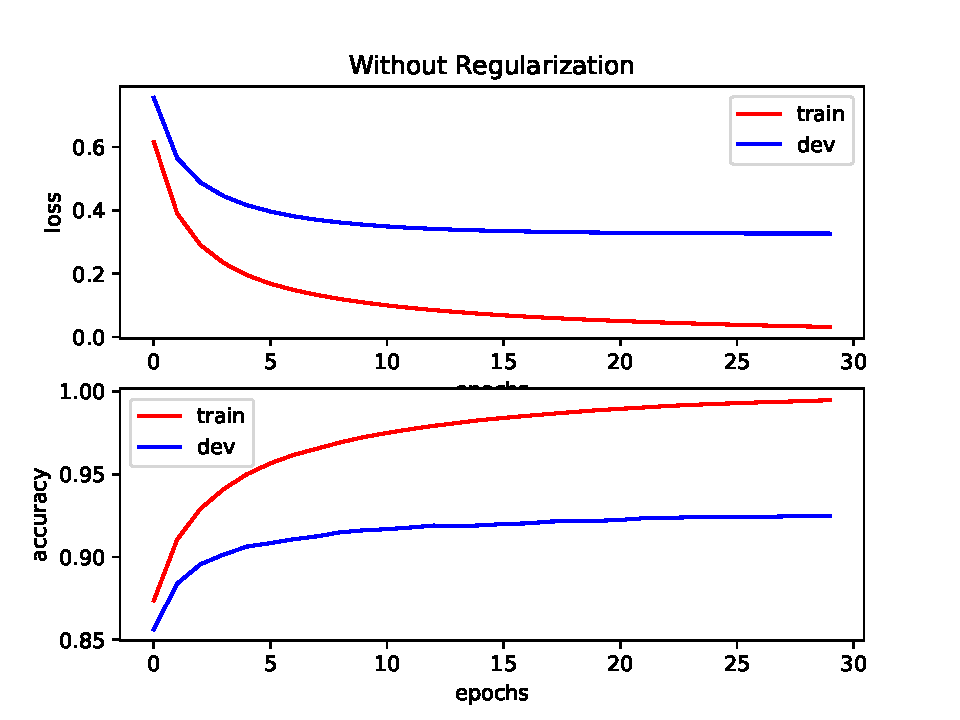
\includegraphics[scale=0.75]{../src/mnist/baseline}

\textbf{Note: \\ Derivation of the gradients for mini-batch gradient descent:}

First, the dimensions of the training data are $X \in \mathbb{R}^{B \times d}$, $y  \in \mathbb{R}^{B \times K}$, and the dimensions of the parameters are $W^{[1]}  \in \mathbb{R}^{d \times h}$, $b^{[1]}  \in \mathbb{R}^{h}$, $W^{[2]}  \in \mathbb{R}^{h \times K}$, $b^{[2]}  \in \mathbb{R}^{K}$.

The forward propagation equations in a vectorized form are:
\begin{align*}
    z^{[1]} &= X W^{[1]} + \tilde{b}^{[1]} &&\in \mathbb{R}^{B \times h}\\
    a &= \sigma \left( z^{[1]} \right) &&\in \mathbb{R}^{B \times h}\\
    z &= a W^{[2]} + \tilde{b}^{[2]} &&\in \mathbb{R}^{B \times K}\\
    \hat{y} &= \text{softmax} \left( z \right) &&\in \mathbb{R}^{B \times K}
\end{align*}
Note that $\tilde{b}$ terms are the broadcasted version of $b$ terms.
For further detail, see the lecture note on Deep learning.

Then, the gradients of $J_{MB}$ with respect to each variable/parameter are:
\begin{align*}
    \nabla_{z} J_{MB} &= \frac{1}{B} \nabla_{z} \mathrm{CE}(y, \hat{y}) &&= \frac{1}{B} \left( \hat{y} - y \right) & &\in \mathbb{R}^{B \times K}\\
    \nabla_{W^{[2]}} J_{MB} &= \frac{1}{B} \nabla_{W^{[2]}} \mathrm{CE}(y, \hat{y}) &&= 
    \frac{1}{B} \underbrace{a^T}_{(h \times B)}  \cdot \underbrace{\left( \hat{y} - y \right)}_{(B \times K)} & &\in \mathbb{R}^{h \times K}\\
    \nabla_{b^{[2]}} J_{MB} &= \frac{1}{B} \nabla_{b^{[2]}} \mathrm{CE}(y, \hat{y}) &&= 
    \frac{1}{B} \underbrace{\vec{\mathbf{1}}}_{(B,)} \cdot \underbrace{\left( \hat{y} - y \right)}_{(B \times K)} & &\in \mathbb{R}^{K}\\
    \nabla_{a} J_{MB} &= \frac{1}{B} \nabla_{a} \mathrm{CE}(y, \hat{y}) &&= 
    \frac{1}{B} \underbrace{\left( \hat{y} - y \right)}_{(B \times K)} \cdot \underbrace{W^{[2]T}}_{(K \times h)} & &\in \mathbb{R}^{B \times h}\\
    \nabla_{z^{[1]}} J_{MB} &= \frac{1}{B} \nabla_{z^{[1]}} \mathrm{CE}(y, \hat{y}) &&= 
    \frac{1}{B} \underbrace{a \odot (1-a)}_{(B \times h)} \odot
    \underbrace{ \left[ \left( \hat{y} - y \right) \cdot W^{[2]T} \right]}_{(B \times h)}
    & &\in \mathbb{R}^{B \times h}\\
    \nabla_{W^{[1]}} J_{MB} &= \frac{1}{B} \nabla_{W^{[1]}} \mathrm{CE}(y, \hat{y}) &&= 
    \frac{1}{B} \underbrace{X^T}_{(d \times B)} \underbrace{ \left[ a \odot (1-a) \odot
    \left( \hat{y} - y \right) \cdot W^{[2]T} \right]}_{(B \times h)} & &\in \mathbb{R}^{d \times h}\\
    \nabla_{b^{[1]}} J_{MB} &= \frac{1}{B} \nabla_{b^{[1]}} \mathrm{CE}(y, \hat{y}) &&= 
    \frac{1}{B} \underbrace{\vec{\mathbf{1}}}_{(B,)} \cdot \underbrace{ \left[ a \odot (1-a) \odot
    \left( \hat{y} - y \right) \cdot W^{[2]T} \right]}_{(B \times h)} & &\in \mathbb{R}^{h}
\end{align*}

\end{answer}
   
  
